\documentclass[11pt]{article}

% Change "review" to "final" to generate the final (sometimes called camera-ready) version.
% Change to "preprint" to generate a non-anonymous version with page numbers.
\usepackage[review]{acl}
\usepackage{pgfplots}
\pgfplotsset{compat=1.18}
\usepackage[colorinlistoftodos,textsize=small]{todonotes}
\newcommand{\inlinetodo}[1]{\todo[inline,color=yellow!40]{\textbf{TODO:} #1}}

% Standard package includes
\usepackage{times}
\usepackage{latexsym}
\usepackage{booktabs}
\usepackage{amsmath}
% For proper rendering and hyphenation of words containing Latin characters (including in bib files)
\usepackage[T1]{fontenc}
% For Vietnamese characters
% \usepackage[T5]{fontenc}
% See https://www.latex-project.org/help/documentation/encguide.pdf for other character sets

% This assumes your files are encoded as UTF8
\usepackage[utf8]{inputenc}

% This is not strictly necessary, and may be commented out,
% but it will improve the layout of the manuscript,
% and will typically save some space.
\usepackage{microtype}

% This is also not strictly necessary, and may be commented out.
% However, it will improve the aesthetics of text in
% the typewriter font.
\usepackage{inconsolata}

%Including images in your LaTeX document requires adding
%additional package(s)
\usepackage{graphicx}

\usepackage{subcaption}
\usepackage{array}
\usepackage{multirow}
\usepackage{amssymb}
\usepackage{enumitem}

% If the title and author information does not fit in the area allocated, uncomment the following
%
%\setlength\titlebox{<dim>}
%
% and set <dim> to something 5cm or larger.

% \title{Instructions for *ACL Proceedings}

% Author information can be set in various styles:
% For several authors from the same institution:
% \author{Author 1 \and ... \and Author n \\
%         Address line \\ ... \\ Address line}
% if the names do not fit well on one line use
%         Author 1 \\ {\bf Author 2} \\ ... \\ {\bf Author n} \\
% For authors from different institutions:
% \author{Author 1 \\ Address line \\  ... \\ Address line
%         \And  ... \And
%         Author n \\ Address line \\ ... \\ Address line}
% To start a separate ``row'' of authors use \AND, as in
% \author{Author 1 \\ Address line \\  ... \\ Address line
%         \AND
%         Author 2 \\ Address line \\ ... \\ Address line \And
%         Author 3 \\ Address line \\ ... \\ Address line}

\title{Analyzing The Impact Of Varying Network Structures On LLM-Based Social Simulations}

%\author{
%  \textbf{First Author\textsuperscript{1}},
%  \textbf{Second Author\textsuperscript{1,2}},
%  \textbf{Third T. Author\textsuperscript{1}},
%  \textbf{Fourth Author\textsuperscript{1}},
%\\
%  \textbf{Fifth Author\textsuperscript{1,2}},
%  \textbf{Sixth Author\textsuperscript{1}},
%  \textbf{Seventh Author\textsuperscript{1}},
%  \textbf{Eighth Author \textsuperscript{1,2,3,4}},
%\\
%  \textbf{Ninth Author\textsuperscript{1}},
%  \textbf{Tenth Author\textsuperscript{1}},
%  \textbf{Eleventh E. Author\textsuperscript{1,2,3,4,5}},
%  \textbf{Twelfth Author\textsuperscript{1}},
%\\
%  \textbf{Thirteenth Author\textsuperscript{3}},
%  \textbf{Fourteenth F. Author\textsuperscript{2,4}},
%  \textbf{Fifteenth Author\textsuperscript{1}},
%  \textbf{Sixteenth Author\textsuperscript{1}},
%\\
%  \textbf{Seventeenth S. Author\textsuperscript{4,5}},
%  \textbf{Eighteenth Author\textsuperscript{3,4}},
%  \textbf{Nineteenth N. Author\textsuperscript{2,5}},
%  \textbf{Twentieth Author\textsuperscript{1}}
%\\
%\\
%  \textsuperscript{1}Affiliation 1,
%  \textsuperscript{2}Affiliation 2,
%  \textsuperscript{3}Affiliation 3,
%  \textsuperscript{4}Affiliation 4,
%  \textsuperscript{5}Affiliation 5
%\\
%  \small{
%    \textbf{Correspondence:} \href{mailto:email@domain}{email@domain}
%  }
%}

\begin{document}
\maketitle
\begin{abstract}
  Generative social simulations use LLM agents to study opinion dynamics, yet the role of the underlying followership network in shaping these dynamics remains under-explored. We systematically study how seven classical graph models---including Erd\H{o}s--R\'enyi, Barab\'asi--Albert, Stochastic Block, and Forest Fire---affect opinion evolution in a multi-agent simulator. In a controlled study of 156 runs holding base model, question, and population size constant, graph topology emerges as a dominant driver of behavior, explaining up to 90.6\% of variance in neighbor-alignment shifts and 28.5\% of consensus-change variance. 385 additional runs vary the base LLM (Gemma, Llama-3.1, Qwen2.5), the survey question, the news agent, and graph density: the topology effect on neighbor alignment survives FDR correction in every condition tested. A complementary 595-run broad exploration with only two topologies yields a near-zero topology signal, showing that between-model variance can mask structural effects in less controlled designs. Network structure is thus a fundamental, not neutral, design choice in LLM social simulations.
\end{abstract}

\section{Introduction}

Social media platforms shape public discourse through the interplay of content and structure: \emph{what} people say matters, but so does \emph{who} follows \emph{whom}. As Large Language Models (LLMs) have developed and gained more agentic capabilities, there has been a surge of interest in systems where multiple LLM agents interact autonomously, from collaborative task-solving \cite{luo2025largelanguagemodelagent} to entirely LLM-populated social-media platforms such as Moltbook \cite{li2026riseaiagentcommunities, zhang2026agentswildsafetysociety}. The field of generative social simulations uses LLMs to simulate humans and their interactions, with one of the end-goals being to simulate human societies and gain insights into sociological phenomena that have historically been hard to study. A key area of research within generative social simulations is social-media simulations. If LLMs can give insights into how humans behave on social media, these systems can be used as sandboxes for a broad array of research \cite{piao2025agentsocietylargescalesimulationllmdriven}. While there have been several proposals for social simulation systems \cite{touzel2024simulationsolvingsocietalscalemanipulation,yang2025oasisopenagentsocial, piao2025agentsocietylargescalesimulationllmdriven}, these lack systematic analyses of their respective components and design choices. In particular, the \emph{followership network}, i.e., the directed graph that determines which agents observe which others' posts, is typically initialized with a single random or unspecified algorithm, with no analysis of how this structural choice affects the resulting dynamics.

Understanding the impact of such network topology choices on generative social simulations is crucial for two primary reasons. First, for researchers utilizing these systems as sociological sandboxes, disentangling the artifacts of the network structure from other components of a simulation is essential to ensure valid conclusions. Second, systematically analyzing the behavior of LLM simulations under different followership-network strategies allows us to get insights into how accurately LLMs approximate human social media behavior. Ultimately, establishing this structural baseline is a necessary foundational step in maturing LLM social simulations. By building a rigorous understanding of these underlying dynamics, these simulated environments can eventually serve as reliable, high-fidelity testbeds for studying malicious disinformation strategies and testing structural interventions, thereby helping to safeguard real-world human online ecosystems \cite{touzel2024simulationsolvingsocietalscalemanipulation}.

In this work, we conduct an empirical study of network topology in LLM social simulations spanning 1136 simulation roll-outs. Our main contributions are:

\begin{itemize}
    \item \textbf{A controlled multi-topology study} (156 runs across seven classical graph models, all other simulation parameters held constant) showing that the followership-network topology is a dominant driver of opinion dynamics, explaining up to 90.6\% of neighbor-alignment variance and 28.5\% of consensus-change variance.
    \item \textbf{Robustness checks across 385 runs} that vary the base LLM (Gemma-3-4B, Llama-3.1-8B, Qwen2.5-7B), the survey question, the news-agent placement, and the graph density: the topology effect on neighbor-alignment shift rate is FDR-significant in every condition tested.
    \item \textbf{A negative-result counterpoint} from a 595-run broad exploration with only two topologies, where strong between-model variance masks the topology signal entirely---highlighting that LLM generative biases must be controlled before structural effects can be reliably detected.
\end{itemize}

\section{Related Works}

Our work lies at the intersection of two primary areas of research: social simulations and network topology algorithms. 

\paragraph{Social Simulators and Opinion Dynamics} \quad Given the promise of social simulations, there have been several works proposing social simulation architectures. These include Oasis \cite{yang2025oasisopenagentsocial} that scales social simulations to 1,000,000 agents and provides some initial work on the evaluation of opinion dynamics such as herding, polarization, and information propagation. Other works, like AgentSociety \cite{piao2025agentsocietylargescalesimulationllmdriven} and SandboxSocial \cite{touzel2024simulationsolvingsocietalscalemanipulation}, also touch on or analyze phenomena such as polarization and opinion evolution. However, none of these works systematically vary the followership network structure, typically relying on a random (or unspecified) network initialization. While there has been some initial work on exploring the effect of network initialization algorithms on opinion dynamics, these have been limited by their scale and design choices. For example, Zheng and Tang \cite{zheng2026simulatingsocialnetwork} provide a preliminary analysis by focusing on the difference between scale-free and small-world networks, but they only conduct studies on a system of 15 agents. Our study expands on such work in three concrete dimensions: scale (up to 4,096 agents), breadth of topologies (seven graph models), and statistical methodology (permutation ANOVA with FDR correction across 1136 total runs).

\paragraph{Network Initialization Algorithms} \quad To understand the impact of topology, the literature traditionally relies on established mathematical baselines to model specific macroscopic network properties. The Erdös-Rényi (ER) model \cite{erdos1959random} provides a foundational baseline of uniform randomness, while Stochastic Block Models (SBM) \cite{abbe2023communitydetectionstochasticblock} are utilized to explicitly construct community structures and study potential echo chambers. Additionally, the Barabási–Albert (BA) model \cite{albert2002statistical}, the Forest Fire (FF) model \cite{leskovec2005graphs}, and directed scale-free graphs \cite{10.5555/644108.644133} have long been the standard for capturing the preferential attachment, dynamic growth, and hub-dominated nature characteristic of real-world social platforms. While more sophisticated approaches have been proposed, our analysis focuses on these classical, widely-used algorithms, which may be expanded by future works.

% For our LLM-based social simulation context, we can also frame the network generation problem as a followership graph prediction problem within a text-attributed graph. Our users are the nodes that possess rich textual personas, and the edges represent the followership relation. Within this framing, previous works have introduced frameworks like GAG-General, provided alongside the GDGB benchmark \cite{peng2026gdgb}. This method treats graph synthesis as an inductive multi-agent simulation task. Additionally, recent empirical studies \cite{10.1093/pnasnexus/pgaf317} demonstrate that when LLMs are allowed to sequentially form links based on textual attributes, they naturally exhibit classical mathematical phenomena like preferential attachment and triadic closure. Yet, the literature also cautions that while LLMs can generate structurally realistic networks that mirror human demographic homophily, they often introduce unique generative artifacts, such as significantly overestimating political homophily \cite{Chang_Chaszczewicz_Wang_Josifovska_Pierson_Leskovec_2025}.

Existing research lacks a systematic empirical analysis of how varying these foundational topologies
%, ranging from classical mathematical algorithms to modern LLM-driven generative artifacts, 
specifically alters the complex, high-dimensional opinion dynamics and information propagation within societies of LLM agents. Our work attempts to bridge this gap, to gain stronger insights into the capabilities of LLM agent-driven social simulations today.

\section{Problem Definition}

In this project, we propose to answer the following research question: \textbf{How does varying the structure of the followership network in an LLM-based social simulation impact opinion dynamics?}

In our experiments, we vary our followership network initialization across seven classical mathematical graph models (see Section \ref{variables_phase_2}). For each algorithm, the followership graph is generated first, and personas are then assigned to nodes, either randomly or using a homophily-aware strategy placing like-minded models together (see Appendix~\ref{appendix_homophily}).

We measure opinion dynamics using several families of metrics. For echo chambers, we use network assortativity, cross-cutting edge fraction, and mean local agreement. For herd effects, we track consensus evolution and the fraction of agents aligning with their neighbors' majority opinion (Neighbor Alignment Shift Rate). For information propagation, we introduce a post-hoc semantic influence analysis: we embed all simulation messages using TwHiN-BERT \cite{zhang2023twhinbertsociallyenrichedpretrainedlanguage} and construct a weighted influence graph where edge weights reflect cosine similarity modulated by temporal decay, allowing us to trace influence cascades and measure global semantic drift across the simulation. As a sanity check for simulation validity, we also include a stylistic realism metric using a BERT classifier.

We hypothesize that the underlying network topology will alter the simulated opinion dynamics. Specifically, we anticipate that (1) hub-dominated topologies (e.g., BA) will facilitate rapid global information propagation but suppress local neighbor-alignment effects, while community-structured topologies (e.g., SBM) will exhibit stronger local clustering of opinion. Furthermore, (2) homophily-aware persona assignment will create measurably different echo-chamber dynamics that interact with the underlying topology.


We note that while many recent works attempt to reproduce human behavior through similar simulation setups, validating claims of human-likeness remains a particularly challenging open question \cite{larooij2025largelanguagemodelssolve}. We will therefore not approach this problem: we are interested in the impact of varying network structure on opinion dynamics in LLM social networks, but make no claims regarding the applicability of our results to human-populated networks.

\section{Dataset}

\paragraph{Pre-existing Data Sources.} The models we use within the simulator are fine-tuned on anonymized BlueSky posts and interactions from the BluePrint dataset \cite{bückkaeffer2025textttblueprintsocialmediauser}. BluePrint clusters users into 25 behavioral archetypes based on posting patterns and topical interests. For each archetype, a Low-Rank Adaptation (LoRA) adapter is trained on that archetype's subset of posts, yielding 25 adapters that capture distinct communication styles and topical tendencies. \inlinetodo{Add 2--3 sentences describing what the 25 archetypes represent (e.g., political orientation, topic focus) and the LoRA training procedure (base model, rank, training data size per archetype).} During simulation, each agent is assigned one of these adapters, which governs its language generation behavior. Survey questions and their per-archetype answer distributions are also sourced from BluePrint. The simulation platform is built by \citet{bückkaeffer2026textitsiliconsocietycookbookdesign}.

\paragraph{Synthetically Generated Data.} The interaction data on which we compute our herd effect, echo chamber, and influence metrics are generated through LLM-based social simulation roll-outs. Given the artificial nature of this dataset, we record all information available within the simulation: the followership graph, regular answers to survey questions, messages written, impressions on each message, messages seen but not interacted-with, and the full observation history per agent. To seed dynamics into the simulation, a biased news agent posts pre-generated ``news'' messages. These were generated using Gemini 3.1 Pro \cite{geminiteam2025geminifamilyhighlycapable}, used from the chat interface, explicitly biased in favor of one survey option, and are loaded from a static set of 50 pre-generated posts per topic.

\section{Methodology}

Our study is centered on a controlled multi-topology experiment (Phase~2, 156 runs, seven graph models, all other simulation parameters held constant), which constitutes the main contribution of the paper. Two supporting analyses surround it: a broad-exploration phase (Phase~1, 595 runs, two topologies, many varied parameters) that motivated Phase~2 with a null result, and a robustness phase (Phase~3, 385 runs) that re-runs the Phase~2 design under varied base models, survey questions, news-agent presence, and graph density. Phase~2 and the headline Phase~3 findings appear in the main body; full Phase~1 results are deferred to Appendix~\ref{appendix:phase1}, and per-condition Phase~3 breakdowns to Appendix~\ref{appendix:robustness_detail}.

\subsection{Metrics}

Designing metrics or evaluations for social simulations can be challenging. This is partly because the imitative nature of the objective makes it hard to define what a realistic simulation means. The literature has yet to converge on a set of metrics, with previous works pointing to the issue of validation remaining poorly addressed and failing to evidence operational validity \cite{larooij2025largelanguagemodelssolve}. To best ground our experimentation, we thus aim to cover a wide range of metrics. 

\paragraph{Realism} We compute a stylistic realism metric by training a BERT classifier to distinguish between human-generated and simulation generated social-media threads. We use the TWHiN model, which was pre-trained on Twitter data \cite{zhang2023twhinbertsociallyenrichedpretrainedlanguage}, as our base, and further train it for our use case. For this purpose, we source human data from the BluePrint dataset and LLM data from our simulation runs. Together, we curate 200000 training samples, carefully avoiding data leakage issues. For each simulation run conducted, 150 threads are used as a test set. If a thread is harder to identify as being AI-generated, we interpret it as being more realistic.

\paragraph{Information Dynamics Metrics} All other metrics are computed using model survey responses. Considering that they lack human baselines, they \textbf{should not} be used to claim that a given set of settings is more realistic than some other. They can, however, be used to measure how each setting impacts the simulation's opinion dynamics, giving us clues regarding which parameters matter most and how they interact. The complete list of metrics is available in Table~\ref{tab:metrics_definitions}. We invite readers to refer to it as needed.

\paragraph{Influence Analysis (Phase 2)} In Phase~2, we additionally compute a post-hoc semantic influence analysis. All simulation messages are embedded using TwHiN-BERT \cite{zhang2023twhinbertsociallyenrichedpretrainedlanguage}, and a weighted influence graph is constructed: for each message, candidate ``parent'' messages are identified from the author's observation history, and edge weights are computed as $w_{ij} \propto \text{cos}(\mathbf{e}_i, \mathbf{e}_j) \cdot \exp(-\beta \cdot \Delta t)$, combining semantic similarity with a Hawkes-process-style temporal decay. Edges exceeding a probability threshold (0.05) are retained as ``filtered'' edges, enabling cascade decomposition and component analysis. Global semantic drift is measured in sliding windows across the simulation timeline. Here, we set $\beta=0.05$.

\subsection{Variables}
\label{variables}

\paragraph{Phase 2 (controlled study).} All Phase~2 runs hold base model, population, question, news agent, proportions, and survey awareness fixed: Llama-3.1-Minitaur-8B as the base model, 256 agents, the AI-copyright question (\ref{appendix_survey_questions}), uniform proportions across 25 LoRAs, one biased news agent placed at the highest-degree node, and survey awareness off. The two varied factors are:
\label{variables_phase_2}

\begin{itemize}
    \item \textbf{Network topology}: seven graph models---Erd\H{o}s--R\'{e}nyi (ER), Barab\'{a}si--Albert (BA), Stochastic Block Model (SBM), cycle, power-law cluster (PLC), fully connected (FC), and Forest Fire (FF). Per-model parameter values are listed in Appendix~\ref{appendix:graph_params}.
    \item \textbf{Homophily}: on or off. When on, agents with similar initial opinions are placed in spatially adjacent nodes (Appendix~\ref{appendix_homophily}).
\end{itemize}

Phase~2 comprises 156 runs (15--27 per topology, 83 with homophily on, 73 off).

\paragraph{Phase 3 (robustness).} A further 385 runs replicate the Phase~2 design while varying, one factor at a time: (i) base LLM among Gemma-3-4B, Llama-3.1-8B, and Qwen2.5-7B-Instruct \cite{binz2025foundation,qwen2,gemma_2025} (210 runs); (ii) survey question among Q25 / Q28 / Q29 (105 runs); (iii) presence vs.\ absence of the news agent (70 runs). All Phase~3 runs use density-controlled graphs ($\approx 16$ mean degree for the five parameterizable topologies; see Appendix~\ref{appendix:graph_params}).

\paragraph{Phase 1 (broad exploration; in appendix).} A 595-run broad-parameter exploration with two topologies (ER and a directed scale-free graph \cite{10.5555/644108.644133}), four base models, four network sizes (64, 256, 1024, 4096 agents), four LoRA-proportion presets, survey awareness on/off, and news agent on/off motivated Phase~2 by producing a near-zero topology effect that we trace to between-model variance dominating the heterogeneous design. Full Phase~1 results, methodology, and variables are in Appendix~\ref{appendix:phase1}. Details on the statistical methodology used throughout the paper are available in Appendix~\ref{appendix:statistical_methods}.


\subsection{Experiment Setup}

Our simulator is taken from \cite{bückkaeffer2026textitsiliconsocietycookbookdesign}. We instantiate a set of agents to populate our simulation and create a followership network connecting them together based on the relevant parameter selected for the run. Agents get attributed an ``action probability'' fixed for the duration of the simulation. At each simulation step, 10 agents are selected according to this action probability. The first 9 observe a recent thread in which someone they follow participated, while the last one has a 1/3 probability of creating a new thread and a 2/3 probability of replying to an already existing one. The simulations run for a total of 2500 steps, with agents surveyed every 250 steps starting at 0 (yielding 11 survey snapshots). Details regarding our choices of parameters are available in the appendix (see \ref{appendix:parameter_justification}). %We select 3 possible survey questions chosen to be maximally divisive (i.e., have agents' answer distributions vary widely, measured using Shannon Entropy).


\section{Results}

\subsection{Controlled Multi-Topology Analysis (156 Runs)}
\label{sec:phase2}

Phase~2 holds all confounding variables constant and expands to seven graph topologies (see Section~\ref{variables_phase_2}). Here, graph topology emerges as an important driver of nearly every metric.

\subsubsection{Behavioral Metrics}

Table~\ref{tab:phase2_behavioral} reports the main results. For each metric, we report the graph-type effect ($\eta^2$ with permutation $p$-value) alongside the homophily effect (Cohen's $d$ with permutation $p$-value), so the two factors are reported on consistent scales. Graph topology explains large and statistically significant variance fractions across all four behavioral metrics.

\begin{table*}[t]
\centering
\begin{tabular}{l cc cc}
\toprule
& \multicolumn{2}{c}{Graph type} & \multicolumn{2}{c}{Homophily} \\
\cmidrule(lr){2-3} \cmidrule(lr){4-5}
Metric & $\eta^2$ & $p_{\text{perm}}$ & $d$ & $p_{\text{perm}}$ \\
\midrule
Net Consensus Change            & 0.285             & $<$0.001 & $+$0.48        & 0.002 \\
Opinion Shift Rate              & 0.219             & $<$0.001 & $+$0.16        & 0.328 \\
Majority Follow Rate            & 0.110             & 0.009    & $+$0.29        & 0.070 \\
Neighbor Alignment Shift Rate   & \textbf{0.906}    & $<$0.001 & $-$0.25        & 0.111 \\
\bottomrule
\end{tabular}
\caption{Phase~2 behavioral metrics. Both factors are reported on consistent scales: $\eta^2$ for graph type (7 levels) and Cohen's $d$ for homophily (2 levels). Permutation $p$-values use 2000 permutations. Graph topology explains large variance fractions, with NASR showing the strongest effect ($\eta^2 = 0.906$). Homophily significantly stabilizes consensus ($d = +0.48$) but does not significantly affect other behavioral metrics. Computed by \texttt{reports/phase2\_analysis.py}.}
\label{tab:phase2_behavioral}
\end{table*}

The most notable result is NASR: graph topology explains 90.6\% of its variance ($p_{\text{perm}} < 0.001$). Table~\ref{tab:topology_attribution} reports per-topology means ($\pm$ standard deviation) across key behavioral and echo metrics. Cycle graphs produce the highest NASR ($0.121 \pm 0.001$) and the strongest consensus erosion (NCC $= -0.150 \pm 0.034$), while Barab\'{a}si--Albert produces the lowest NASR ($0.068 \pm 0.006$) and fully connected graphs show the least erosion (NCC $= -0.064 \pm 0.034$). For net consensus change, both topology ($\eta^2 = 0.285$) and homophily ($d = +0.48$, $p_{\text{perm}} = 0.002$) are significant. We separate the Erd\H{o}s--R\'enyi row in Table~\ref{tab:topology_attribution} because it is the default initialization used in most existing social-simulation work; it sits in the middle of the topology ordering for every metric. Full per-topology means including initial/final values, exposure diversity, same-option exposure, all echo-chamber metrics, and all temporal deltas are in Appendix Tables~\ref{tab:appendix_behavioral_per_topo}, \ref{tab:appendix_echo_per_topo}, and \ref{tab:appendix_delta_per_topo}.

\begin{table*}[t]
\centering
\small
\begin{tabular}{l c cccccc}
\toprule
Topology & $n$ & NCC & NASR & OSR & MFR & Final Asst. & Local Agr. \\
\midrule
Cycle            & 24 & $-$0.150$\pm$0.034 & \textbf{0.121$\pm$0.001} & 0.253$\pm$0.009 & 0.474$\pm$0.006 & \textbf{0.155$\pm$0.172} & \textbf{0.582$\pm$0.090} \\
Forest Fire      & 15 & $-$0.080$\pm$0.033 & 0.115$\pm$0.007 & 0.244$\pm$0.014 & 0.492$\pm$0.016 & $-$0.003$\pm$0.002 & 0.527$\pm$0.017 \\
Fully Connected  & 18 & \textbf{$-$0.064$\pm$0.034} & 0.113$\pm$0.002 & 0.245$\pm$0.003 & 0.488$\pm$0.005 & $-$0.001$\pm$0.001 & 0.548$\pm$0.017 \\
Stoch.\ Block    & 25 & $-$0.121$\pm$0.036 & 0.098$\pm$0.006 & \textbf{0.259$\pm$0.009} & 0.484$\pm$0.020 & 0.032$\pm$0.039 & 0.525$\pm$0.022 \\
PL Cluster       & 22 & $-$0.112$\pm$0.038 & 0.091$\pm$0.006 & 0.255$\pm$0.011 & 0.488$\pm$0.012 & 0.001$\pm$0.014 & 0.528$\pm$0.020 \\
Barab\'{a}si--Albert & 25 & $-$0.132$\pm$0.039 & 0.068$\pm$0.006 & 0.255$\pm$0.008 & 0.485$\pm$0.020 & 0.024$\pm$0.029 & 0.538$\pm$0.026 \\
\midrule
\multicolumn{8}{l}{\textit{Default in existing literature:}} \\
Random (ER)      & 27 & $-$0.106$\pm$0.062 & 0.095$\pm$0.007 & 0.255$\pm$0.010 & 0.488$\pm$0.020 & 0.017$\pm$0.026 & 0.531$\pm$0.048 \\
\bottomrule
\end{tabular}
\caption{Per-topology means $\pm$ standard deviation for behavioral and echo-chamber metrics (Phase~2, $n=156$). NCC: Net Consensus Change; NASR: Neighbor Alignment Shift Rate; OSR: Opinion Shift Rate; MFR: Majority Follow Rate; Final Asst.: final assortativity; Local Agr.: final local agreement. Random (ER) is separated as the default topology used by most existing social-simulation work. All metrics show significant graph-type effects ($p_{\text{perm}} \leq 0.009$). Full metric breakdown with initial values, deltas, and other echo metrics is in Appendix~\ref{appendix:per_topology_full}. Computed by \texttt{reports/phase2\_analysis.py}.}
\label{tab:topology_attribution}
\end{table*}

We note, however, that NASR's construction makes it partly mechanically sensitive to topology. In a cycle graph, the minimal two-neighbor structure means any opinion shift is very likely to match one neighbor's opinion, inflating NASR relative to denser topologies. In a fully connected graph, the ``neighbor majority'' collapses to the global majority, making NASR and MFR conceptually equivalent. The $\eta^2 = 0.906$ for NASR therefore reflects both genuine behavioral differences and this structural sensitivity. NCC ($\eta^2 = 0.285$), which aggregates consensus at the population level without reference to neighborhood structure, provides the more conservative and topology-neutral estimate of the behavioral impact of graph structure.

\begin{figure}[t]
\centering
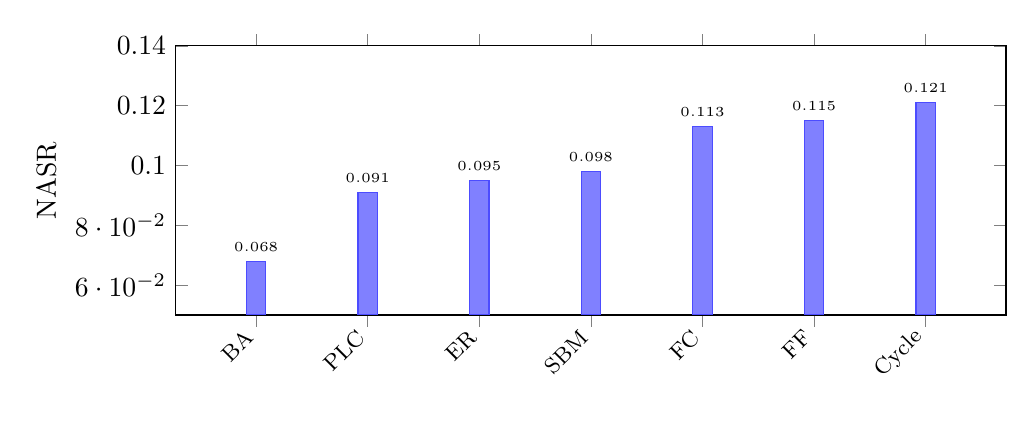
\begin{tikzpicture}
\begin{axis}[
    ybar,
    bar width=7pt,
    width=\columnwidth,
    height=5cm,
    ylabel={NASR},
    symbolic x coords={BA, PLC, ER, SBM, FC, FF, Cycle},
    xtick=data,
    x tick label style={rotate=45, anchor=east, font=\footnotesize},
    ymin=0.05, ymax=0.14,
    ytick={0.06, 0.08, 0.10, 0.12, 0.14},
    nodes near coords,
    nodes near coords style={font=\tiny, /pgf/number format/fixed, /pgf/number format/precision=3},
    enlarge x limits=0.12,
]
\addplot[fill=blue!50, draw=blue!70] coordinates {
    (BA, 0.068) (PLC, 0.091) (ER, 0.095) (SBM, 0.098) (FC, 0.113) (FF, 0.115) (Cycle, 0.121)
};
\end{axis}
\end{tikzpicture}
\caption{Per-topology NASR means in Phase~2, ordered by increasing NASR. BA = Barab\'{a}si--Albert, PLC = Power-law Cluster, ER = Erd\H{o}s--R\'{e}nyi, SBM = Stochastic Block Model, FC = Fully Connected, FF = Forest Fire. The 77\% relative range between BA (0.068) and Cycle (0.121) illustrates the practical impact of topology choice.}
\label{fig:nasr_topology}
\end{figure}

\subsubsection{Echo-Chamber Metrics}
\label{sec:phase2_echo}

In Phase~2, both topology and homophily produce large, significant effects on echo-chamber structure (Table~\ref{tab:phase2_echo}). The temporal deltas show that homophily-initialized networks undergo substantial structural change:

\begin{itemize}
    \item $\Delta$ assortativity: $-0.002$ (no homophily) vs.\ $-0.194$ (homophily), $d = -1.90$
    \item $\Delta$ local agreement: $-0.066$ vs.\ $-0.144$, $d = -1.35$
    \item $\Delta$ cross-cutting edges: $+0.063$ vs.\ $+0.151$, $d = +1.60$
\end{itemize}

\begin{table*}[t]
\centering
\begin{tabular}{l cc cc}
\toprule
& \multicolumn{2}{c}{Graph type} & \multicolumn{2}{c}{Homophily} \\
\cmidrule(lr){2-3} \cmidrule(lr){4-5}
Metric & $\eta^2$ & $p_{\text{perm}}$ & $d$ & $p_{\text{perm}}$ \\
\midrule
Final assortativity   & 0.363 & $<$0.001 & $+$0.81 & $<$0.001 \\
Final local agreement & 0.166 & $<$0.001 & $+$1.13 & $<$0.001 \\
Final cross-cutting   & 0.218 & $<$0.001 & $-$0.99 & $<$0.001 \\
Exposure diversity    & 0.308 & $<$0.001 & $-$0.50 & 0.001 \\
\bottomrule
\end{tabular}
\caption{Phase~2 echo-chamber metrics (final snapshot), reported on consistent effect-size scales. Both factors produce significant effects. Homophily effects are very large (Cohen's $d$ up to 1.13). Computed by \texttt{reports/phase2\_analysis.py}.}
\label{tab:phase2_echo}
\end{table*}

Graph topology also significantly modulates these temporal changes (all $\Delta$ metrics show graph $p_{\text{perm}} \leq 0.002$). As shown in Table~\ref{tab:topology_attribution}, cycle graphs exhibit the largest assortativity decay ($\Delta = -0.225$), while fully connected graphs remain nearly stable ($\Delta = +0.002$). This indicates that LLM agents do not simply preserve the opinion clustering imposed at initialization; they shift opinions in ways that erode echo-chamber structure. Hub-dominated topologies partially resist this erosion by concentrating influence through a small number of highly connected nodes, which may act to repeatedly reinforce the dominant local opinion. Topologies with more uniform connectivity allow more diverse opinion signals to reach each agent, accelerating the breakdown of initial clustering.

\subsubsection{Influence Metrics}
\label{sec:phase2_influence}

The semantic influence analysis reveals that topology shapes information-flow (Table~\ref{tab:phase2_influence}).

\begin{table*}[t]
\centering
\begin{tabular}{l cc cc}
\toprule
& \multicolumn{2}{c}{Graph type} & \multicolumn{2}{c}{Homophily} \\
\cmidrule(lr){2-3} \cmidrule(lr){4-5}
Metric & $\eta^2$ & $p_{\text{perm}}$ & $d$ & $p$ (FDR $q$) \\
\midrule
Influence edge count & 0.855 & $<$0.001 & $-$0.62 & 0.0004 \\
Filtered edge count  & 0.919 & $<$0.001 & ---     & 0.071 \\
Filtered-edge rate   & 0.697 & $<$0.001 & $+$0.92 & $<$0.001 \\
Cascade roots        & 0.287 & $<$0.001 & ---     & 0.073 \\
Global drift mean    & 0.289 & $<$0.001 & $+$0.38 & 0.020 \\
\bottomrule
\end{tabular}
\caption{Phase~2 influence metrics. Graph topology is the dominant factor, explaining 85.5--91.9\% of variance in edge-based influence measures. Computed by \texttt{src/influence\_metrics.py}.}
\label{tab:phase2_influence}
\end{table*}

Graph topology accounts for up to 91.9\% of the variance in filtered edge count (i.e. the number of high-confidence influence relationships). Homophily significantly increases the filtered-edge rate ($d = 0.92$): when agents start with similar-minded neighbors, a greater proportion of influence edges exceed the significance threshold. This could be because like-minded agents influence each-other more, but it is also possible that our measurement method misinterprets preexisting agreement for causal influence. As shown in Table~\ref{tab:topology_attribution}, stochastic block and random graphs have the highest filtered-edge rates (0.0235), while fully connected graphs have the lowest (0.0212). Forest fire graphs produce the highest global semantic drift (0.111), while cycle graphs produce the lowest (0.103).

\subsubsection{Cross-Domain Correlations}

The influence metrics correlate meaningfully with behavioral outcomes.

Higher filtered-edge rates (more concentrated influence pathways) are associated with greater opinion shift rate ($r = 0.465$, $p < 10^{-10}$), consistent with both metrics being proxies of inter-agent influence. Higher global semantic drift correlates with net consensus change ($r = 0.482$, $p < 10^{-11}$), which suggests that our embedding-based semantic metrics do capture opinions to a degree. The negative correlation between the largest influence component size and net consensus change ($r = -0.297$, $p < 10^{-4}$) suggests that when information propagates through a single large cascade, it may concentrate opinion pressure in ways that reduce diversity. Together, these correlations support the interpretation that topology affects behavioral outcomes in part by shaping the structure of information flow.

\subsection{Robustness (385 Runs)}
\label{sec:phase3}

Phase~3 re-runs the Phase~2 design under varied conditions to test the generalizability of the topology effect: 210 runs replicate Phase~2 across three additional LLM families (Gemma-3-4B, Llama-3.1-8B, Qwen2.5-7B), 105 runs cover three survey questions (Q25, Q28, Q29), and 70 runs remove the biased news agent. All Phase~3 runs use density-controlled graphs ($\approx 16$ mean degree for the five parameterizable topologies). Across all 48 hypothesis tests, we apply Benjamini--Hochberg FDR correction at $\alpha = 0.05$.

Table~\ref{tab:robustness_summary} summarises the headline result: the NASR topology effect survives FDR correction at $q < 0.01$ in every condition tested. Effect sizes range from $\eta^2 = 0.400$ (Qwen) to $\eta^2 = 0.835$ (no-news), all substantially lower than Phase~2's $\eta^2 = 0.906$ but still large. NCC topology effects do not survive FDR correction for any of the three new LLMs, consistent with our finding (also confirmed in Phase~1) that base-model identity dominates NCC variance. Within the five parameterizable topologies, density does not significantly predict NASR ($r = 0.063$, $q = 0.364$), so the topology effect within this group is structural rather than density-driven. The per-topology NASR ordering is qualitatively stable across questions (Kendall $\tau = 1.0$ for Q28 vs.\ Q29) and across LLM families ($\tau = 0.52$--$0.62$ between model pairs). Removing the news agent has no significant effect on NASR ($\Delta = +0.003$, $d = 0.18$, $q = 0.483$) but does increase NCC and OSR, consistent with the news agent acting as a persistent opinion broadcaster orthogonal to local neighbor dynamics. BERT realism does not significantly vary by topology after FDR correction ($q = 0.089$), confirming that the behavioral differences are not driven by differential text realism. Per-condition statistical breakdowns, per-topology means under each condition, and the full 48-test FDR registry are in Appendix~\ref{appendix:robustness_detail}.

\begin{table}[t]
\centering
\small
\begin{tabular}{l c c c c}
\toprule
Condition & $N$ & $\eta^2_{\text{NASR}}$ & $q$ & $\eta^2_{\text{NCC}}$ \\
\midrule
Phase~2 (Minitaur, ref.) & 156 & 0.906 & --- & 0.285 \\
\midrule
Gemma-3-4B   & 77 & 0.785 & 0.003 & 0.098\textsuperscript{ns} \\
Llama-3.1-8B & 57 & 0.599 & 0.003 & 0.163\textsuperscript{ns} \\
Qwen2.5-7B   & 76 & 0.400 & 0.006 & 0.162\textsuperscript{ns} \\
\midrule
Q25 & 31 & 0.734 & 0.003 & 0.501* \\
Q28 (ctrl) & 32 & 0.736 & 0.003 & 0.409\textsuperscript{ns} \\
Q29 & 42 & 0.570 & 0.003 & 0.321\textsuperscript{ns} \\
\midrule
No news agent & 70 & 0.835 & 0.003 & 0.238* \\
\bottomrule
\end{tabular}
\caption{NASR and NCC topology effect sizes across the 8 robustness conditions. All NASR effects are FDR-significant ($q < 0.01$). NCC effects marked with * survive FDR correction; \textsuperscript{ns} indicates the effect did not survive correction. The Phase~2 row is the reference condition (uncorrected, single battery).}
\label{tab:robustness_summary}
\end{table}

\section{Discussion}
\label{sec:discussion}

\subsection{LLM Generative Biases as a Confound}

The failure of Phase~1 (Appendix~\ref{appendix:phase1}) to detect topology effects is as informative as Phase~2's strong detections. In Phase~1's heterogeneous design, between-model variance dominates: consensus levels range from 0.993 (Qwen on Q28) to 0.562 (Gemma on Q29), and this LLM-specific variation dwarfs any structural signal from just two topology types. The practical implication is that LLM generative biases must be treated as a confound and controlled for before structural effects can be reliably measured. This is an inherent challenge for simulation studies that vary multiple parameters simultaneously: a null topology result in a heterogeneous design is not evidence that topology does not matter, but may simply reflect that the topology signal is masked. Phase~2's strong effects ($\eta^2$ up to 0.906) emerge only once this confound is removed; Phase~3 then partially recovers generalizability by replicating the controlled design across three additional LLM families.

\subsection{Topology as a Non-Neutral Design Choice}

For researchers using LLM-based social simulations as sociological sandboxes, the attribution results in Table~\ref{tab:topology_attribution} carry a direct practical message: topology initialization is not a neutral design decision. Across otherwise identical conditions, NASR varies by almost a factor of two between the lowest (BA, 0.068) and highest (cycle, 0.121) topology, and consensus erosion varies by more than a factor of two. A simulation built on a BA graph will produce qualitatively different dynamics from one built on a cycle or fully connected graph, and reported findings will reflect this choice whether or not the researcher intends them to. Studies that do not justify and conduct sensitivity analysis over their topology choice risk drawing conclusions that are specific to that initialization.

The homophily erosion results add a related concern. Researchers who design experiments to study echo-chamber formation or persistence may find that LLM agents are structurally non-persistent: initial opinion clustering degrades substantially over the simulation ($d = -1.90$ for $\Delta$ assortativity), even though homophily leaves a residual signal in final metrics. Studies that measure only final snapshots will underestimate the degree of structural change. Whether this erosion reflects a limitation of current LLM architectures, agents rationally updating on diverse content, or a property of the specific simulator's survey mechanism remains an open question, but it is a property researchers should be aware of when interpreting results.

\subsection{Influence Analysis as a Diagnostic Tool}

The post-hoc semantic influence pipeline introduced here proved capable of capturing topology-dependent information-flow patterns that correlate with behavioral outcomes. The fact that these correlations are significant ($r = 0.465$, $r = 0.482$) and topology-dependent suggests that influence-derived metrics provide complementary information to survey-response metrics. This pipeline is general: it operates on message embeddings and temporal metadata, making it applicable to other LLM simulation frameworks that record message histories. Applying it across frameworks could help identify whether topology-behavior coupling is specific to this simulator or a broader property of LLM social dynamics.

\subsection{Future Work}

%The most immediate extension is a multi-model Phase~2 replication to assess whether topology effects generalize across LLM families. 
Testing LLM-driven graph generation methods (e.g., GAG-General) would situate classical mathematical topologies relative to learned ones and test whether LLM-generated graphs introduce distinct interaction patterns. Longer simulations would clarify whether echo-chamber erosion is a transient or persistent phenomenon. Finally, introducing a recommendation algorithm as a structural layer above the followership graph would more closely replicate real social media architectures, and its interaction with static topology effects would be informative for simulation design.

\section{Conclusions}

We investigated how network topology affects opinion dynamics in LLM-based social simulations through a 1136-run empirical study. Our key findings are:

\begin{enumerate}
    \item \textbf{Topology is the dominant driver of opinion dynamics} when confounding variables are controlled. Graph type explains up to 90.6\% of variance in neighbor-alignment behavior and 28.5\% of consensus change variance.

    \item \textbf{The topology effect is robust across LLM families, survey questions, and news-agent presence.} The 385-run Phase~3 confirms that the NASR topology effect survives FDR correction in every condition tested ($q < 0.01$), and is not driven by graph density within the parameterizable group.

    \item \textbf{LLM generative biases must be controlled before structural effects can be detected.} The 595-run Phase~1 broad exploration (Appendix~\ref{appendix:phase1}) shows near-zero topology effects, because between-model variance masks the structural signal. This has direct implications for the design of future LLM simulation studies.

    \item \textbf{Homophily creates echo-chamber structure that systematically erodes.} Homophily-initialized networks show large initial clustering effects ($d$ up to 1.13) that decay substantially ($d = -1.90$ for $\Delta$ assortativity), with erosion rate modulated by topology.
\end{enumerate}

Together, these findings establish that network topology is a fundamental design parameter in LLM social simulations, not a neutral initialization choice. Future work can delve further into these phenomena.

\section{Limitations}

%\paragraph{Single base model in Phase~2.} Phase~2 uses only Llama-3.1-Minitaur-8B. While this controls for between-model variance, the results may not generalize to other LLM families. The strong Phase~1 evidence that base model explains more behavioral variance than topology in heterogeneous settings underscores this caveat. Similar comments are true of other parameters we fixed in Phase~2.

\paragraph{News-agent placement.} The biased news agent is placed at the highest-degree node in all runs. Because degree centrality differs across topologies, the news agent's reach is not constant across conditions. However, topology effects are consistent across both homophily conditions and across metrics where the news agent has no direct causal pathway (e.g., NASR is computed from survey responses), suggesting that topology effects are not solely driven by news-agent reach.

\paragraph{Simulation duration.} At 2500 steps with 10 agents per step, Phase~2's 256-agent runs yield roughly 97 actions per agent. Longer simulations might clarify whether the observed echo-chamber erosion is a transient warm-up effect or a stable long-run property. However, due to time, scope, and resource constraints, we don't conduct this analysis here.

\paragraph{LLM-driven topologies. and Deep-Learning based Topologies} We do not test LLM-driven graph generation methods such as GAG-General \cite{peng2026gdgb}, or deep-learning generated topology structures. These may show other significant and interesting variations in comparison to our setup. Our study remains limited to classical network generation algorithms.


\section{Ethical Considerations}

Our work studies how network structure shapes opinion dynamics in simulated social environments. The intended application is to inform the design of more rigorous LLM social simulations. In general, malicious actors typically can't control network structures in social media. As such, we don't expect strong dual-use concerns. However, we acknowledge that insights about how network topology amplifies or suppresses opinion shifts could, in principle, inform the design of more effective manipulation campaigns on real social platforms. We believe that understanding these structural dynamics is a necessary prerequisite for developing effective countermeasures, and that the controlled, artificial nature of our simulations (using LLM agents with synthetic personas, not real users) limits direct transferability. Nonetheless, researchers building on this work should consider dual-use implications and prioritize defensive applications.

\bibliography{EMNLP_submission/custom}


\appendix
\section{Appendix}

\subsection{Homophily-aware Agent Placement}
\label{appendix_homophily}

When homophily is enabled, we use the spatial-opinion alignment strategy introduced by \citet{bückkaeffer2026textitsiliconsocietycookbookdesign}, in which the assignment of personas to nodes is biased so that graph neighbors tend to share initial opinions. The procedure interleaves a structural ordering of the graph with an ideological ordering of the agents, then assigns them via the resulting rank.

Concretely: (i) we run a 2D Fruchterman--Reingold spring layout on the graph and project nodes onto the $x$-axis to obtain a one-dimensional ordering of the network's structural regions---connected nodes end up near each other on this axis; (ii) for each LoRA persona, we score its expected opinion as the dot product of its survey-answer distribution and an ordinal coding of the answer options (e.g., ``Strongly Disagree''~$\to$~0, $\ldots$, ``Strongly Agree''~$\to$~4); (iii) we sort the agent population by this expected-opinion score, producing an ``ideological spectrum''; (iv) we align the two orderings rank-by-rank, mapping the leftmost spatial node to the lowest-opinion agent and the rightmost to the highest. Because the spring layout colocates connected nodes in Euclidean space, this mapping makes graph neighbors substantially more likely to share initial opinions, producing the structural homophily required to study echo-chamber dynamics. When homophily is disabled, agents are instead mapped to nodes by a uniformly random permutation seeded by the run identifier.

\subsection{Metrics}

\begin{table*}[h]
\centering
\small
\begin{tabular}{|l|c|p{5.8cm}|c|}
\hline
\textbf{Metric} & \textbf{Acronym} & \textbf{Explanation} & \textbf{Formula} \\ \hline
\multicolumn{4}{|l|}{\textit{Behavioral (Herd Effect) Metrics}} \\ \hline
Consensus & --- & The proportion of the population holding the most popular opinion at a specific time step. & $\frac{N_{\max}}{N_{\text{total}}}$ \\ \hline
Net Consensus Change & NCC & The total convergence or divergence of the population over the entire simulation. & $C_{t_f} - C_{t_0}$ \\ \hline
Opinion Shift Rate & OSR & The fraction of the population that changed their opinion between consecutive survey snapshots. & $\frac{N_{\text{changed}}}{N_{\text{total}}}$ \\ \hline
Majority Follow Rate & MFR & Of agents who changed their minds, the fraction that adopted the current global majority opinion. & $\frac{N_{\text{changed} \to \text{maj}}}{N_{\text{changed}}}$ \\ \hline
Neighbor Alignment Shift Rate & NASR & The fraction of the total population that changed their opinion to match the majority of their direct social neighbors. & $\frac{N_{\text{changed} \to \text{nb\_maj}}}{N_{\text{total}}}$ \\ \hline
\multicolumn{4}{|l|}{\textit{Echo-Chamber (Structural) Metrics}} \\ \hline
Assortativity & --- & The tendency of agents to be connected to others with the same opinion (Network Assortativity Coefficient). & $\frac{\text{Tr}(\mathbf{e}) - \lVert \mathbf{e}^2 \rVert}{1 - \lVert \mathbf{e}^2 \rVert}$ \\ \hline
Local Agreement & --- & On average, what fraction of an agent's neighbors share the same opinion. & $\frac{1}{N}\sum_{i}\frac{|\{j \in \mathcal{N}_i : o_j = o_i\}|}{|\mathcal{N}_i|}$ \\ \hline
Cross-Cutting Edge Fraction & --- & The fraction of edges connecting agents who hold different opinions. & $\frac{|\{(i,j) \in E : o_i \neq o_j\}|}{|E|}$ \\ \hline
Exposure Diversity & --- & Mean Shannon entropy of the opinion distribution in threads each agent observed. & $\frac{1}{N}\sum_i H(\mathbf{p}_i)$ \\ \hline
\multicolumn{4}{|l|}{\textit{Influence Metrics (Phase 2 only)}} \\ \hline
Filtered-Edge Rate & --- & The proportion of influence graph edges exceeding a probability threshold, indicating strong semantic influence. & $\frac{|E_{\text{filtered}}|}{|E_{\text{total}}|}$ \\ \hline
Global Semantic Drift & --- & Mean cosine-distance drift of messages from their exposure context, measured in sliding windows. & $\bar{d}_{\text{window}}$ \\ \hline
\end{tabular}
\caption{Behavioral, structural, and influence metrics. Influence metrics are computed post-hoc using TwHiN-BERT embeddings (Phase~2 only).}
\label{tab:metrics_definitions}
\end{table*}

\subsection{Survey questions}
\label{appendix_survey_questions}

The question we ask models in the simulations is one of the following
\begin{enumerate}
    \item Should it be legal to use copyrighted material to train artificial intelligence models? You may only answer with 'Yes' or 'No'.
    \item Is it acceptable to use genetic engineering to enhance human intelligence? You may only answer with 'Yes' or 'No'.
    \item Would you rather vote for a candidate who prioritizes economic growth over environmental protection, or a candidate who prioritizes environmental protection over economic growth? You may only answer with 'Economic Growth' or 'Environmental Protection'.
\end{enumerate}

These questions are taken from \citet{bückkaeffer2026textitsiliconsocietycookbookdesign}.

\subsection{Graph-generation algorithm parameters}
\label{appendix:graph_params}

All graphs are generated by \texttt{src/main.py} using the parameters listed below. Phase~2 and Phase~3 share these settings, except that Phase~3 was explicitly designed to control the mean degree of the five parameterizable topologies (ER, BA, SBM, PL Cluster, Forest Fire) to approximately 16, so the topology effect cannot be attributed to differences in edge count. Cycle (mean degree 2) and fully connected (mean degree $N-1$) cannot be density-matched by construction.

\paragraph{Phase~3 (density-controlled, $\approx 16$ mean degree).}
\begin{itemize}[leftmargin=*]
    \item \textbf{Erd\H{o}s--R\'enyi}: \texttt{nx.erdos\_renyi\_graph(N, p)} with $p = 1/16$; expected mean degree $= (N-1)/16 \approx 16.0$.
    \item \textbf{Power-law Cluster}: \texttt{nx.powerlaw\_cluster\_graph(N, m, p)} with $m = 8$, $p_{\text{tri}} = 0.4$.
    \item \textbf{Barab\'{a}si--Albert}: \texttt{nx.barabasi\_albert\_graph(N, m)} with $m = 8$.
    \item \textbf{Stochastic Block Model}: 4 balanced blocks ($\approx N/4$ nodes each); $p_{\text{in}} = 0.17$, $p_{\text{out}} = 0.028$.
    \item \textbf{Forest Fire}: a custom undirected forest-fire generator with forward burn probability $0.21$ and a cap of $4$ burn visits per new node.
    \item \textbf{Cycle}: \texttt{nx.cycle\_graph(N)}, mean degree $= 2$.
    \item \textbf{Fully Connected}: \texttt{nx.complete\_graph(N)}, mean degree $= N-1$.
\end{itemize}

For all topologies above, $N = 257$ (256 agents + 1 news agent for Phase~3 ``with news'' conditions; otherwise $N = 256$).

\paragraph{Phase~2 graphs.} Phase~2 was run before density was explicitly controlled. The above parameters were also used for the parameterizable topologies, with observed mean degrees of $15.34$--$16.10$ across ER, BA, SBM, and PL Cluster, and a wider $5.46$--$34.40$ for Forest Fire (since the forest-fire process has stochastic spread). See Table~\ref{tab:density_summary} for empirical density statistics aggregated across the Phase~3 runs.

\begin{table}[h]
\centering
\small
\begin{tabular}{l r r r r r}
\toprule
Topology & $n$ runs & Mean deg.\ & SD & Min & Max \\
\midrule
Cycle           & 54 &   2.00 & 0.00 &   2.00 &   2.00 \\
Forest Fire     & 56 &  15.82 & 8.00 &   5.46 &  34.40 \\
Fully Connected & 54 & 255.84 & 0.38 & 255.00 & 256.00 \\
Stoch.\ Block   & 59 &  16.10 & 0.34 &  15.36 &  16.84 \\
Random (ER)     & 59 &  16.06 & 0.32 &  15.24 &  17.06 \\
PL Cluster      & 56 &  15.34 & 0.04 &  15.26 &  15.40 \\
Barab\'{a}si--Albert & 47 &  15.50 & 0.00 &  15.50 &  15.50 \\
\bottomrule
\end{tabular}
\caption{Empirical mean degree of generated graphs across Phase~3 runs. The five parameterizable topologies are matched to a target mean degree of $\approx 16$; Forest Fire has the widest spread because its generative process is stochastic. Computed by \texttt{reports/reviewer\_response\_analysis.py}.}
\label{tab:density_summary}
\end{table}

\subsection{Parameter Justification} 
\label{appendix:parameter_justification}
Using BluePrint \cite{bückkaeffer2025textttblueprintsocialmediauser}, we find that, on average, users post 24.3 messages per month. With 2500 steps and 10 agents acting per step, the simulation produces approximately 25,000 total actions. For 256 agents (Phase~2), this yields roughly 97 actions per agent, sufficient for multiple opinion-revision opportunities. For Phase~1's larger networks (1024 or 4096 agents), per-agent action counts drop to roughly 24 and 6 respectively, which we acknowledge as a limitation at larger scales (see Section~\ref{sec:discussion}). Each simulation runs on either an A100 or an RTX8000 GPU and takes between 2 and 16 hours to complete.

\subsection{Statistical Methods}
\label{appendix:statistical_methods}
In Phase~1, effects are tested using Welch's $t$-tests (normal approximation) with a conservative threshold of $p \leq 0.01$ to guard against multiple comparisons. In Phase~2, we adopt a multi-factor framework: graph-type effects (7 groups) are tested using one-way ANOVA $F$-statistics with permutation $p$-values (2000 permutations); homophily effects use a two-sample permutation test on the mean difference (also 2000 permutations). Both factors are reported on consistent scales ($\eta^2$ and Cohen's $d$, respectively). In Phase~3, all 48 hypothesis tests are jointly corrected using Benjamini--Hochberg FDR ($\alpha = 0.05$). Phase~2 statistics are reproduced by \texttt{reports/phase2\_analysis.py}; Phase~3 statistics by \texttt{reports/reviewer\_response\_analysis.py}.

\subsection{Robustness (Phase 3): Per-Condition Detail}
\label{appendix:robustness_detail}

This appendix provides the per-condition breakdown of the 385 Phase~3 runs summarised in the main body (Table~\ref{tab:robustness_summary}). All Phase~3 runs hold every other Phase~2 condition fixed except the listed variable, and use density-controlled graphs (Appendix~\ref{appendix:graph_params}).

\subsubsection{Multi-Model Generalization}

We replicate Phase~2 across three additional LLM families: Gemma-3-4B, Llama-3.1-8B, and Qwen2.5-7B-Instruct (210 runs total, 7 topologies $\times$ 2 homophily conditions $\times$ $\approx$5 replications each). The NASR topology effect is FDR-significant for every model tested ($q < 0.01$; Table~\ref{tab:robustness_summary}). Effect sizes range from $\eta^2 = 0.400$ (Qwen) to $\eta^2 = 0.785$ (Gemma), all substantially lower than Phase~2's $\eta^2 = 0.906$ but still large. The per-topology ordering is qualitatively stable across models: cycle and fully connected graphs consistently produce the highest NASR, while power-law cluster and BA consistently rank lowest (Kendall $\tau$ = 0.52--0.62 between model pairs; see Appendix~\ref{appendix:robustness_detail} for full per-topology means). NCC topology effects do not survive FDR correction for any of the three new models, consistent with Phase~1's finding that base model dominates NCC variance. The NASR topology conclusion extends across LLM families; the NCC conclusion remains model-dependent.

\subsubsection{Density Control}

Within the five parameterizable topologies (ER, BA, SBM, power-law cluster, Forest Fire), all matched to approximately 16 mean degree, density does not significantly predict NASR ($r = 0.063$, $q = 0.364$). Forest Fire has the widest density range (mean degree 5.46--34.40, SD = 8.00) and still shows no within-topology density-NASR association ($r = 0.105$, $q = 0.507$). These results indicate that topology effects within the parameterizable group are driven by structural properties (clustering, community organization, preferential attachment) rather than edge count. Cycle (mean degree 2) and fully connected (mean degree $N - 1$) cannot be density-matched by construction; their behavioral extremes are consistent with structural rather than density-driven explanations. Full density measurements are reported in Appendix~\ref{appendix:robustness_detail}.

\subsubsection{Stylistic Realism}

TwHiN-BERT classifier accuracy across topologies, using density-controlled baseline runs ($n = 32$), averages 0.902 (SD = 0.035), ranging from 0.872 (fully connected) to 0.933 (Forest Fire). After FDR correction, topology does not significantly modulate realism ($F = 2.78$, $q = 0.089$). This confirms that the behavioral differences reported across topologies are not confounded by differential text realism.

\subsubsection{Cross-Question Robustness}

We replicate Phase~2 across three survey questions: Q25 (genetic enhancements), Q28 (AI copyright), and Q29 (environmental protection), totaling 105 runs. Initial conditions differ substantially: Q25 and Q28 start at moderate majority ($\approx$ 0.56), while Q29 starts at full consensus (1.000). Despite these differences, the NASR topology effect is FDR-significant for all three questions ($q = 0.003$ each; $\eta^2$ = 0.734, 0.736, 0.570 respectively). The per-topology NASR ordering is highly consistent: the Q28--Q29 rank correlation is perfect (Kendall $\tau = 1.0$, $q = 0.008$), and Q25 pairs show $\tau = 0.714$ ($q = 0.061$). The Q29 floor effect compresses absolute NASR values (range 0.018--0.027) but does not disrupt the relative topology ordering, confirming that the NASR topology mechanism operates independently of the question's initial distribution.

\subsubsection{News-Agent Ablation}

We conduct 70 runs without any news agent, all other Phase~2 conditions held constant. The NASR topology effect remains large and FDR-significant ($\eta^2 = 0.835$, $q = 0.003$). Direct comparison with news-agent runs confirms that the news agent has no significant effect on NASR ($\Delta = 0.003$, $q = 0.483$, $d = 0.18$) but does significantly raise NCC ($d = 0.57$, $q = 0.031$) and OSR ($d = 0.72$, $q = 0.008$). This dissociation is expected: NASR measures alignment with direct social neighbors, a structural property independent of a single broadcaster node, while NCC and OSR are population-level aggregates sensitive to persistent opinion pressure. The most notable per-topology shift without the news agent is BA, whose NASR increases from 0.068 to 0.093, consistent with the news agent's high-degree placement monopolizing the BA hub's information environment (see Appendix~\ref{appendix:robustness_detail} for full per-topology comparison).
\paragraph{Phase 3 batches.} The three Phase~3 batches and their purposes are summarised in Table~\ref{tab:phase3_batches}. Per-batch ANOVAs are in Tables~\ref{tab:phase3_model_anova}, \ref{tab:phase3_question_anova}, and \ref{tab:phase3_nonews_anova}. Per-topology NASR means broken down by model are in Table~\ref{tab:phase3_per_topology_models}. Rank-correlation diagnostics are in Tables~\ref{tab:phase3_rank_models} and \ref{tab:phase3_rank_questions}. Density correlations are in Table~\ref{tab:phase3_density_corr}. Initial-consensus differences across questions are in Table~\ref{tab:phase3_init_consensus}. News-vs-no-news direct comparisons are in Table~\ref{tab:phase3_news_vs_nonews}. BERT topology accuracy is in Table~\ref{tab:phase3_bert}.

\begin{table*}[h]
\centering
\small
\begin{tabular}{llcl}
\toprule
Batch & Purpose & $N$ runs & Variable \\
\midrule
\texttt{emnlp2026model}    & Multi-model robustness  & 210 & Base model: Gemma-3-4B, Llama-3.1-8B, Qwen2.5-7B \\
\texttt{emnlp2026question} & Cross-question check    & 105 & Survey question: Q25, Q28, Q29 \\
\texttt{emnlp2026nonews}   & News-agent ablation     & 70  & No news agent (vs.\ 1 in Phase~2) \\
\texttt{emnlp\_visualizer\_baseline} & Density-controlled Phase~2 analogue & 32 & Q28, Minitaur \\
\bottomrule
\end{tabular}
\caption{Phase~3 robustness batches. Loaded by \texttt{reports/reviewer\_response\_analysis.py}.}
\label{tab:phase3_batches}
\end{table*}

\begin{table*}[h]
\centering
\small
\begin{tabular}{llccccc}
\toprule
Model & Metric & $F$ & $\eta^2$ & $p$ (perm) & $q$ (BH) & sig.\ \\
\midrule
Gemma     & NASR & 42.7 & 0.785 & $<$0.001 & 0.003 & ** \\
Gemma     & NCC  & 1.26 & 0.098 & 0.291    & 0.364 & ns \\
Gemma     & OSR  & 1.29 & 0.099 & 0.255    & 0.350 & ns \\
Gemma     & MFR  & 2.28 & 0.163 & 0.045    & 0.089 & ns \\
Llama-3.1 & NASR & 12.4 & 0.599 & $<$0.001 & 0.003 & ** \\
Llama-3.1 & NCC  & 1.63 & 0.163 & 0.159    & 0.231 & ns \\
Llama-3.1 & OSR  & 1.90 & 0.186 & 0.094    & 0.158 & ns \\
Llama-3.1 & MFR  & 2.03 & 0.196 & 0.077    & 0.138 & ns \\
Qwen      & NASR & 7.65 & 0.400 & $<$0.001 & 0.006 & ** \\
Qwen      & NCC  & 2.22 & 0.162 & 0.043    & 0.089 & ns \\
Qwen      & OSR  & 4.36 & 0.275 & 0.001    & 0.008 & ** \\
Qwen      & MFR  & 1.76 & 0.133 & 0.121    & 0.181 & ns \\
\bottomrule
\end{tabular}
\caption{Per-model topology ANOVAs across all four behavioural metrics. NASR survives FDR correction for every LLM family tested; NCC and MFR do not, consistent with the broader finding that base model dominates NCC variance.}
\label{tab:phase3_model_anova}
\end{table*}

\begin{table*}[h]
\centering
\small
\begin{tabular}{lllll}
\toprule
Topology & Phase~2 (Minitaur) & Gemma & Llama-3.1 & Qwen \\
\midrule
Cycle             & \textbf{0.121}     & \textbf{0.114} ($n=9$)  & 0.073 ($n=7$)  & 0.061 ($n=8$)  \\
Forest Fire       & 0.115              & 0.077 ($n=9$)           & 0.062 ($n=6$)  & 0.047 ($n=17$) \\
Fully Connected   & 0.113              & 0.111 ($n=8$)           & \textbf{0.085} ($n=5$) & 0.049 ($n=13$) \\
Stoch.\ Block     & 0.098              & 0.092 ($n=9$)           & 0.076 ($n=15$) & \textbf{0.070} ($n=8$) \\
Random (ER)       & 0.095              & 0.094 ($n=15$)          & 0.075 ($n=5$)  & 0.051 ($n=13$) \\
PL Cluster        & 0.091              & 0.077 ($n=15$)          & 0.063 ($n=10$) & 0.048 ($n=9$)  \\
Barab\'{a}si--Albert & \textbf{0.068}  & 0.078 ($n=12$)          & 0.065 ($n=9$)  & 0.050 ($n=8$)  \\
\bottomrule
\end{tabular}
\caption{Per-topology NASR means by base model. The ordering is qualitatively stable across models (Cycle / Fully Connected at the top, PL Cluster / BA at the bottom).}
\label{tab:phase3_per_topology_models}
\end{table*}

\begin{table*}[h]
\centering
\small
\begin{tabular}{lcccc}
\toprule
Pair & Spearman $r_s$ & Kendall $\tau$ & $p$ & $q$ (BH) \\
\midrule
Gemma vs Llama-3.1 & 0.750 & 0.619 & 0.051 & 0.094 \\
Gemma vs Qwen      & 0.643 & 0.524 & 0.099 & 0.158 \\
Llama-3.1 vs Qwen  & 0.607 & 0.524 & 0.099 & 0.158 \\
\bottomrule
\end{tabular}
\caption{Rank-ordering consistency of the per-topology NASR mean across LLM families. With only 7 topology levels, Kendall $\tau$ requires near-perfect agreement to reach FDR significance; the point estimates are nonetheless substantive and directionally consistent.}
\label{tab:phase3_rank_models}
\end{table*}

\subsubsection{Cross-Question and Density Tables}

\begin{table}[h]
\centering
\small
\begin{tabular}{lccl}
\toprule
Question & $N$ & Initial consensus & Notes \\
\midrule
Q25 (genetic enhancements)     & 31 & $0.566 \pm 0.000$ & Moderate majority \\
Q28 (AI copyright)             & 32 & $0.555 \pm 0.015$ & Moderate majority \\
Q29 (environmental protection) & 42 & $1.000 \pm 0.000$ & Full consensus at $t=0$ \\
\bottomrule
\end{tabular}
\caption{Initial consensus by survey question (Phase~3 question batch).}
\label{tab:phase3_init_consensus}
\end{table}

\begin{table*}[h]
\centering
\small
\begin{tabular}{llccccc}
\toprule
Q & Metric & $F$ & $\eta^2$ & $p$ (perm) & $q$ (BH) & sig.\ \\
\midrule
Q25 & NASR & 11.0 & 0.734 & $<$0.001 & 0.003 & ** \\
Q25 & NCC  &  4.0 & 0.501 & 0.008    & 0.031 & * \\
Q25 & OSR  &  2.8 & 0.410 & 0.042    & 0.089 & ns \\
Q25 & MFR  & 0.67 & 0.144 & 0.685    & 0.730 & ns \\
Q28 & NASR & 13.9 & 0.736 & $<$0.001 & 0.003 & ** \\
Q28 & NCC  &  3.5 & 0.409 & 0.019    & 0.054 & ns \\
Q28 & OSR  &  1.3 & 0.205 & 0.287    & 0.364 & ns \\
Q28 & MFR  &  1.0 & 0.167 & 0.444    & 0.507 & ns \\
Q29 & NASR &  7.7 & 0.570 & $<$0.001 & 0.003 & ** \\
Q29 & NCC  &  2.8 & 0.321 & 0.027    & 0.065 & ns \\
Q29 & OSR  & 0.58 & 0.090 & 0.748    & 0.780 & ns \\
Q29 & MFR  & 0.93 & 0.138 & 0.514    & 0.574 & ns \\
\bottomrule
\end{tabular}
\caption{Per-question topology ANOVAs. NASR effects are FDR-significant for all three questions ($q = 0.003$ each).}
\label{tab:phase3_question_anova}
\end{table*}

\begin{table}[h]
\centering
\small
\begin{tabular}{lcccc}
\toprule
Pair & Spearman $r_s$ & Kendall $\tau$ & $p$ & $q$ (BH) \\
\midrule
Q25 vs Q28 & 0.857 & 0.714 & 0.024 & 0.061 \\
Q25 vs Q29 & 0.857 & 0.714 & 0.024 & 0.061 \\
Q28 vs Q29 & \textbf{1.000} & \textbf{1.000} & \textbf{0.002} & \textbf{0.008} \\
\bottomrule
\end{tabular}
\caption{NASR rank-ordering consistency across questions. The Q28/Q29 ordering is identical.}
\label{tab:phase3_rank_questions}
\end{table}

\begin{table}[h]
\centering
\small
\begin{tabular}{lcccc}
\toprule
Test & $r$ & $p$ & $q$ (BH) & $n$ \\
\midrule
FF density vs NASR                          & 0.105 & 0.438 & 0.507 & 56 \\
FF density vs NCC                           & 0.172 & 0.200 & 0.283 & 56 \\
All 5 param.\ topologies: density vs NASR   & 0.063 & 0.296 & 0.364 & 277 \\
\bottomrule
\end{tabular}
\caption{Density--NASR correlation tests within the parameterizable topologies. None significant after FDR correction.}
\label{tab:phase3_density_corr}
\end{table}

\subsubsection{News-Agent Ablation Tables}

\begin{table}[h]
\centering
\small
\begin{tabular}{lccccc}
\toprule
Metric & $F$ & $\eta^2$ & $p$ (perm) & $q$ (BH) & sig.\ \\
\midrule
NASR & 53.0 & \textbf{0.835} & $<$0.001 & \textbf{0.003} & ** \\
NCC  &  3.3 & 0.238          & 0.009    & \textbf{0.031} & * \\
OSR  &  3.3 & 0.237          & 0.011    & \textbf{0.037} & * \\
MFR  &  1.8 & 0.146          & 0.106    & 0.165          & ns \\
\bottomrule
\end{tabular}
\caption{No-news topology ANOVAs ($n=70$). NASR/NCC/OSR topology effects all survive FDR correction.}
\label{tab:phase3_nonews_anova}
\end{table}

\begin{table}[h]
\centering
\small
\begin{tabular}{lccccc}
\toprule
Metric & With news & No news & $\Delta$ & $p$ & $q$ (BH) \\
\midrule
NASR & 0.109 ($n=32$) & 0.106 ($n=70$) & $+$0.003 & 0.403 & 0.483 \\
NCC  & 0.055 ($n=32$) & 0.027 ($n=70$) & $+$0.028 & 0.008 & 0.031 \\
OSR  & 0.280 ($n=32$) & 0.272 ($n=70$) & $+$0.008 & 0.002 & 0.008 \\
\bottomrule
\end{tabular}
\caption{Direct news vs.\ no-news comparison on the density-controlled Q28 baseline. The news agent leaves NASR essentially unchanged but raises NCC and OSR, consistent with its role as a population-level opinion broadcaster.}
\label{tab:phase3_news_vs_nonews}
\end{table}

\subsubsection{BERT Realism}

\begin{table}[h]
\centering
\small
\begin{tabular}{lccc}
\toprule
Topology & $N$ & Mean BERT acc.\ & SD \\
\midrule
Cycle                & 6 & 0.911 & 0.030 \\
Forest Fire          & 4 & 0.933 & 0.028 \\
Fully Connected      & 6 & 0.872 & 0.043 \\
Stoch.\ Block        & 3 & 0.885 & 0.021 \\
Random (ER)          & 6 & 0.889 & 0.034 \\
PL Cluster           & 6 & 0.920 & 0.018 \\
Barab\'{a}si--Albert & 1 & 0.922 & --- \\
\textbf{Overall}     & \textbf{32} & \textbf{0.902} & \textbf{0.035} \\
\bottomrule
\end{tabular}
\caption{TwHiN-BERT human-vs-LLM classification accuracy per topology on the density-controlled Q28 baseline. Topology effect: $F=2.78$, $p=0.046$, $q=0.089$ (ns after FDR). Average accuracy is uniformly high ($>0.87$), so behavioural topology effects are not confounded by differential text realism.}
\label{tab:phase3_bert}
\end{table}

% =====================================================================
\subsection{Per-Topology Full Metric Breakdown (Phase 2)}
\label{appendix:per_topology_full}
% =====================================================================

This appendix expands Table~\ref{tab:topology_attribution} from the main body with all behavioural, echo-chamber, and temporal-delta metrics. All values are computed by \texttt{reports/phase2\_analysis.py} from the 156 Phase~2 runs, reported as mean $\pm$ standard deviation. Initial consensus is constant ($0.699 \pm 0.000$) across all topologies because Phase~2 fixes the LoRA proportions and question.

\begin{table*}[h]
\centering
\small
\begin{tabular}{lcccccc}
\toprule
Topology & $n$ & NCC & NASR & OSR & MFR & Final cons.\ \\
\midrule
Cycle               & 24 & $-$0.150$\pm$0.034 & 0.121$\pm$0.001 & 0.253$\pm$0.009 & 0.474$\pm$0.006 & 0.549$\pm$0.034 \\
Forest Fire         & 15 & $-$0.080$\pm$0.033 & 0.115$\pm$0.007 & 0.244$\pm$0.014 & 0.492$\pm$0.016 & 0.619$\pm$0.033 \\
Fully Connected     & 18 & $-$0.064$\pm$0.034 & 0.113$\pm$0.002 & 0.245$\pm$0.003 & 0.488$\pm$0.005 & 0.635$\pm$0.034 \\
Stoch.\ Block       & 25 & $-$0.121$\pm$0.036 & 0.098$\pm$0.006 & 0.259$\pm$0.009 & 0.484$\pm$0.020 & 0.578$\pm$0.036 \\
PL Cluster          & 22 & $-$0.112$\pm$0.038 & 0.091$\pm$0.006 & 0.255$\pm$0.011 & 0.488$\pm$0.012 & 0.587$\pm$0.038 \\
Barab\'{a}si--Albert & 25 & $-$0.132$\pm$0.039 & 0.068$\pm$0.006 & 0.255$\pm$0.008 & 0.485$\pm$0.020 & 0.567$\pm$0.039 \\
\midrule
Random (ER)         & 27 & $-$0.106$\pm$0.062 & 0.095$\pm$0.007 & 0.255$\pm$0.010 & 0.488$\pm$0.020 & 0.593$\pm$0.062 \\
\bottomrule
\end{tabular}
\caption{Behavioural metrics per topology, Phase~2 (mean $\pm$ SD). Random (ER) is separated as the default initialization in existing work.}
\label{tab:appendix_behavioral_per_topo}
\end{table*}

\begin{table*}[h]
\centering
\small
\begin{tabular}{lcccccc}
\toprule
Topology & Init.\ Asst.\ & Final Asst.\ & Init.\ Loc.\ Agr.\ & Final Loc.\ Agr.\ & Init.\ Cross-cut.\ & Exposure div.\ \\
\midrule
Cycle               & 0.381$\pm$0.375    & 0.155$\pm$0.172   & 0.739$\pm$0.158 & 0.582$\pm$0.090 & 0.261$\pm$0.158 & 0.429$\pm$0.013 \\
Forest Fire         & $-$0.002$\pm$0.002 & $-$0.003$\pm$0.002 & 0.578$\pm$0.009 & 0.527$\pm$0.017 & 0.422$\pm$0.000 & 0.476$\pm$0.015 \\
Fully Connected     & $-$0.003$\pm$0.001 & $-$0.001$\pm$0.001 & 0.576$\pm$0.008 & 0.548$\pm$0.017 & 0.422$\pm$0.000 & 0.476$\pm$0.017 \\
Stoch.\ Block       & 0.158$\pm$0.167    & 0.032$\pm$0.039   & 0.646$\pm$0.068 & 0.525$\pm$0.022 & 0.354$\pm$0.078 & 0.447$\pm$0.016 \\
PL Cluster          & 0.092$\pm$0.078    & 0.001$\pm$0.014   & 0.647$\pm$0.053 & 0.528$\pm$0.020 & 0.367$\pm$0.059 & 0.451$\pm$0.015 \\
Barab\'{a}si--Albert & 0.179$\pm$0.136   & 0.024$\pm$0.029   & 0.689$\pm$0.084 & 0.538$\pm$0.026 & 0.330$\pm$0.081 & 0.440$\pm$0.013 \\
\midrule
Random (ER)         & 0.086$\pm$0.109    & 0.017$\pm$0.026   & 0.617$\pm$0.056 & 0.531$\pm$0.048 & 0.384$\pm$0.055 & 0.443$\pm$0.046 \\
\bottomrule
\end{tabular}
\caption{Echo-chamber metrics per topology, Phase~2 (mean $\pm$ SD). ``Init.''\ is the first survey snapshot; ``Final''\ is the last. Final cross-cutting equals $1-$ final local agreement and is omitted.}
\label{tab:appendix_echo_per_topo}
\end{table*}

\begin{table*}[h]
\centering
\small
\begin{tabular}{lcccc}
\toprule
Topology & $\Delta$ Asst.\ & $\Delta$ Loc.\ Agr.\ & $\Delta$ Cross-cut.\ & $\Delta$ Same-opt.\ Exp.\ \\
\midrule
Cycle               & $-$0.225$\pm$0.203 & $-$0.157$\pm$0.068 & $+$0.157$\pm$0.068 & $+$0.512$\pm$0.008 \\
Forest Fire         & $-$0.000$\pm$0.002 & $-$0.051$\pm$0.017 & $+$0.050$\pm$0.016 & $+$0.532$\pm$0.019 \\
Fully Connected     & $+$0.002$\pm$0.000 & $-$0.028$\pm$0.024 & $+$0.041$\pm$0.019 & $+$0.541$\pm$0.005 \\
Stoch.\ Block       & $-$0.126$\pm$0.138 & $-$0.121$\pm$0.058 & $+$0.120$\pm$0.062 & $+$0.518$\pm$0.012 \\
PL Cluster          & $-$0.091$\pm$0.075 & $-$0.119$\pm$0.049 & $+$0.121$\pm$0.055 & $+$0.521$\pm$0.017 \\
Barab\'{a}si--Albert & $-$0.155$\pm$0.128 & $-$0.151$\pm$0.072 & $+$0.153$\pm$0.078 & $+$0.512$\pm$0.010 \\
\midrule
Random (ER)         & $-$0.069$\pm$0.098 & $-$0.086$\pm$0.059 & $+$0.087$\pm$0.058 & $+$0.529$\pm$0.052 \\
\bottomrule
\end{tabular}
\caption{Temporal deltas (final $-$ initial survey snapshot) per topology, Phase~2 (mean $\pm$ SD). Negative $\Delta$ assortativity and $\Delta$ local agreement indicate erosion of initial opinion clustering over the simulation.}
\label{tab:appendix_delta_per_topo}
\end{table*}

% =====================================================================
\subsection{Phase 1: Broad Exploration (595 Runs)}
\label{appendix:phase1}
% =====================================================================

This appendix details the Phase~1 broad-exploration runs that motivated the controlled Phase~2 design.

\paragraph{Variables.} Phase~1 varies eight parameters simultaneously: two network topologies (Erd\H{o}s--R\'enyi and a directed scale-free graph \cite{10.5555/644108.644133}); four network sizes (64, 256, 1024, 4096 agents); four base models (Llama-3.1-Minitaur-8B, Llama-3.1-8B, Qwen2.5-7B-Instruct, gemma-3-4b-pt); on/off homophily; on/off ``survey awareness'' (whether each agent can see its own prior survey answers); on/off biased news agent; four LoRA-proportion presets; and three survey questions (Appendix~\ref{appendix_survey_questions}). Phase~1 comprises 595 simulation roll-outs with randomized parameter combinations.

\subsubsection{Behavioral Effects Are Near-Zero}

Across the headline behavioural outcomes, both topology and homophily have small, non-significant effects (Table~\ref{tab:main_effects_near_zero}). With only two topology types and many confounding factors pooled, neither network topology nor homophily materially alters the magnitude of social dynamics (opinion volatility, herding, or consensus change) in cross-sectional comparisons.

\begin{table*}[h]
\centering
\begin{tabular}{lcc}
\toprule
Metric & Graph type effect (random $-$ powerlaw) & Homophily effect (True $-$ False) \\
\midrule
Net Consensus Change & $-0.014$ ($p = 0.230$, $d = -0.10$) & $+0.004$ ($p = 0.716$, $d = +0.03$) \\
Opinion Shift Rate   & $+0.013$ ($p = 0.168$, $d = +0.11$) & $-0.003$ ($p = 0.775$, $d = -0.02$) \\
Majority Follow Rate & $-0.008$ ($p = 0.422$, $d = -0.07$) & $-0.004$ ($p = 0.725$, $d = -0.03$) \\
NASR                 & $+0.004$ ($p = 0.212$, $d = +0.10$) & $-0.002$ ($p = 0.601$, $d = -0.04$) \\
\bottomrule
\end{tabular}
\caption{Phase~1 main effects of graph type and homophily on behavioural metrics are small and non-significant. Numbers reproduced by \texttt{reports/verify\_report\_numbers.py}.}
\label{tab:main_effects_near_zero}
\end{table*}

\subsubsection{Echo-Chamber Structure and Temporal Dynamics}

Echo-chamber metrics show sensitivity to homophilic initialization but no correlation with graph type:
\begin{itemize}
    \item Final assortativity by homophily: $0.0059$ (True) vs.\ $-0.0040$ (False), $\Delta = +0.0099$, $p = 0.004$, $d = 0.24$.
    \item Graph type on final assortativity: $p = 0.375$ (ns).
    \item Final local agreement, cross-cutting edges, and same-option exposure: all graph type and homophily contrasts ns ($p \geq 0.20$).
\end{itemize}
Homophily leaves a small positive residual in final opinion assortativity (an expected sanity check: assortativity directly measures opinion homophily). The strongest Phase~1 effects appear in \textit{time-series deltas} (last $-$ first survey step), especially for assortativity (Table~\ref{tab:temporal_dynamics}). Cell means for $\Delta$ assortativity show a non-linear interaction (Table~\ref{tab:delta_assortativity_vs_homophily}): the interaction contrast is $IC = +0.0382$, confirming that power-law topology dampens the homophily-driven assortativity collapse, but only when homophily is active.

\begin{table*}[h]
\centering
\begin{tabular}{lcc}
\toprule
Delta metric & Graph type effect (random $-$ powerlaw) & Homophily effect (True $-$ False) \\
\midrule
$\Delta$ assortativity        & $-0.0165$ ($p = 0.016$, $d = -0.20$) & $\mathbf{-0.0486}$ ($p < 0.001$, $d = -0.62$) \\
$\Delta$ local agreement      & $-0.0152$ ($p = 0.225$, ns)          & $-0.0163$ ($p = 0.193$, ns) \\
$\Delta$ cross-cutting edges  & $+0.0133$ ($p = 0.290$, ns)          & $+0.0179$ ($p = 0.155$, ns) \\
\bottomrule
\end{tabular}
\caption{Phase~1 temporal-delta effects. Homophily significantly reduces assortativity over time; other temporal effects are small.}
\label{tab:temporal_dynamics}
\end{table*}

\begin{table}[h]
\centering
\begin{tabular}{lcc}
\toprule
Homophily & False & True \\
\midrule
random   & $+0.0021$ & $-0.0671$ \\
powerlaw & $+0.0023$ & $-0.0286$ \\
\bottomrule
\end{tabular}
\caption{Phase~1: $\Delta$ assortativity by homophily and topology. Power-law topology partially dampens the homophily-driven assortativity decay.}
\label{tab:delta_assortativity_vs_homophily}
\end{table}

\subsubsection{Interpreting the Phase~1 Null}

The near-zero behavioural effects admit several explanations: (a) between-model variance dominates: different base models yield very different consensus levels (e.g., Qwen on Q28 at 0.993 vs.\ Gemma on Q29 at 0.562), so pooling across four models masks within-topology effects; (b) limited topological contrast---with only two graph types, neither specifically designed to produce community structure, the topological variation may be insufficient; (c) per-agent action counts at the largest network sizes (roughly 6 actions per agent at $N = 4096$) may be too few for structural effects to propagate over the simulation horizon. These considerations directly motivated the controlled design of Phase~2.

\end{document}
